\let\negmedspace\undefined
\let\negthickspace\undefined
\documentclass[journal]{IEEEtran}
\usepackage[a5paper, margin=10mm, onecolumn]{geometry}
\usepackage{lmodern} % Ensure lmodern is loaded for pdflatex
\usepackage{tfrupee} % Include tfrupee package

\setlength{\headheight}{1cm} % Set the height of the header box
\setlength{\headsep}{0mm}     % Set the distance between the header box and the top of the text

\usepackage{gvv-book}
\usepackage{gvv}
\usepackage{cite}
\usepackage{amsmath,amssymb,amsfonts,amsthm}
\usepackage{algorithmic}
\usepackage{graphicx}
\usepackage{textcomp}
\usepackage{xcolor}
\usepackage{txfonts}
\usepackage{listings}
\usepackage{enumitem}
\usepackage{mathtools}
\usepackage{gensymb}
\usepackage{comment}
\usepackage[breaklinks=true]{hyperref}
\usepackage{tkz-euclide} 
\usepackage{listings}
\usepackage{gvv}                                        
\def\inputGnumericTable{}                                 
\usepackage[latin1]{inputenc}                                
\usepackage{color}                                            
\usepackage{array}                                            
\usepackage{longtable}                                       
\usepackage{calc}                                             
\usepackage{multirow}                                         
\usepackage{hhline}                                           
\usepackage{ifthen}                                           
\usepackage{lscape}  
\usetikzlibrary{patterns}
\begin{document}
\bibliographystyle{IEEEtran}
\begin{center}
    \textbf{\Large GATE(2023)}
    
    \textbf{Biomedical Engineering (BM)}
    
    \vspace{0.5cm}
    \textbf{General Aptitude (GA)}
    \end{center}

    \textbf{Q.1 - Q.5 Carry ONE mark Each}

\begin{enumerate}
   
 \item \quad ``I cannot support this proposal. My \underline{\hspace{3cm}} will not permit it.''
 
\hfill (GATE BM 2023

\begin{enumerate}
    \item conscious
    \item consensus
    \item conscience
    \item consent
    
\end{enumerate}


\item  \quad Courts : \underline{\hspace{2cm}} : Parliament : Legislature\\
(By word meaning)

<<<<<<< HEAD
\hfill{\brak{\text{GATE PE 2016}}}
=======
\hfill{\brak{\text{GATE BM 2023}}}
>>>>>>> b031c34efd4dd324facb86a5e10db7b7cbd90dc1

\begin{enumerate}
    \item Judiciary
    \item Executive
    \item Governmental
    \item Legal
\end{enumerate}


 \item What is the smallest number with distinct digits whose digits add up to 45?

<<<<<<< HEAD
\hfill{\brak{\text{GATE PE 2016}}}
=======
\hfill{\brak{\text{GATE BM 2023}}}
>>>>>>> b031c34efd4dd324facb86a5e10db7b7cbd90dc1

\begin{enumerate}
    \item 123555789
    \item 123457689
    \item 123456789
    \item 99999
\end{enumerate}


\item 
In a class of 100 students,
\begin{enumerate}
    \item there are 30 students who neither like romantic movies nor comedy movies,
    \item the number of students who like romantic movies is twice the number of students who like comedy movies, and
    \item the number of students who like both romantic movies and comedy movies is 20.
\end{enumerate}

How many students in the class like romantic movies?
<<<<<<< HEAD
\hfill{\brak{\text{GATE PE 2016}}}
=======
\hfill{\brak{\text{GATE BM 2023}}}
>>>>>>> b031c34efd4dd324facb86a5e10db7b7cbd90dc1

\begin{enumerate}
    \item 40
    \item 20
    \item 60
    \item 30
\end{enumerate}
<<<<<<< HEAD
\hfill{\brak{\text{GATE PE 2016}}}
=======
\hfill{\brak{\text{GATE BM 2023}}}
>>>>>>> b031c34efd4dd324facb86a5e10db7b7cbd90dc1

\newpage
\item  
How many rectangles are present in the given figure?
\begin{figure}[H]
    \centering
    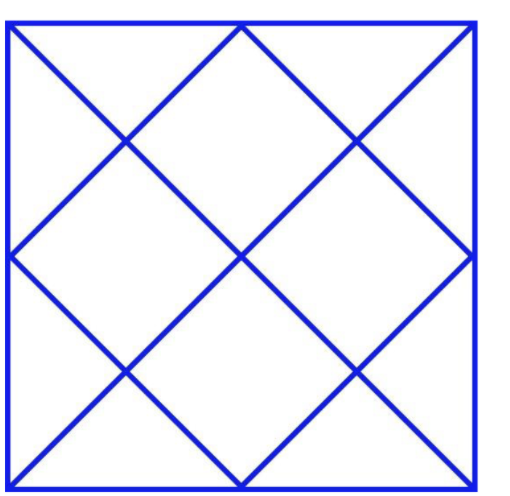
\includegraphics[width=0.4\columnwidth]{Figs/Q5}
    \caption{}
    \label{}
\end{figure}

\begin{enumerate}
    \item 8
    \item 9
    \item 10
    \item 12
\end{enumerate}
<<<<<<< HEAD
\hfill{\brak{\text{GATE PE 2016}}}
=======
\hfill{\brak{\text{GATE BM 2023}}}
>>>>>>> b031c34efd4dd324facb86a5e10db7b7cbd90dc1

\section*{Q.6 - Q.10 Carry TWO marks Each}

\item 
Forestland is a planet inhabited by different kinds of creatures. Among other creatures, it is populated by animals all of whom are ferocious. There are also creatures that have claws, and some that do not. All creatures that have claws are ferocious.



Based only on the information provided above, which one of the following options can be logically inferred with \textit{certainty}?

<<<<<<< HEAD
\hfill{\brak{\text{GATE PE 2016}}}
=======
\hfill{\brak{\text{GATE BM 2023}}}
>>>>>>> b031c34efd4dd324facb86a5e10db7b7cbd90dc1

\begin{enumerate}
    \item All creatures with claws are animals.
    \item Some creatures with claws are non-ferocious.
    \item Some non-ferocious creatures have claws.
    \item Some ferocious creatures are creatures with claws.
\end{enumerate}

\item 
Which one of the following options represents the given graph?

<<<<<<< HEAD
\hfill{\brak{\text{GATE PE 2016}}}

\begin{center}
\begin{tikzpicture}[scale=1.2]
  \draw[->] (-4,0) -- (4,0) node[right] {$x$};
  \draw[->] (0,-0.5) -- (0,4) node[above] {$f(x)$};
  \draw[domain=-3.5:3.5, smooth, variable=\x, blue, thick] 
    plot ({\x}, {(\x)^2 * 2^(-abs(\x))});
  \foreach \x in {-3,-2,-1,1,2,3}
    \draw (\x,0.1) -- (\x,-0.1) node[below] {\x};
  \foreach \y in {1,2,3}
    \draw (0.1,\y) -- (-0.1,\y) node[left] {\y};
\end{tikzpicture}
\end{center}

\begin{enumerate}
    \item[(A)] \( f(x) = x^2 \cdot 2^{-|x|} \)
    \item[(B)] \( f(x) = x \cdot 2^{-|x|} \)
    \item[(C)] \( f(x) = |x| \cdot 2^{-x} \)
    \item[(D)] \( f(x) = x \cdot 2^{-x} \)
     \end{enumerate}
     \hfill{\brak{\text{GATE PE 2016}}}
     
=======
\hfill{\brak{\text{GATE BM 2023}}}
\begin{figure}[H]
    \centering
    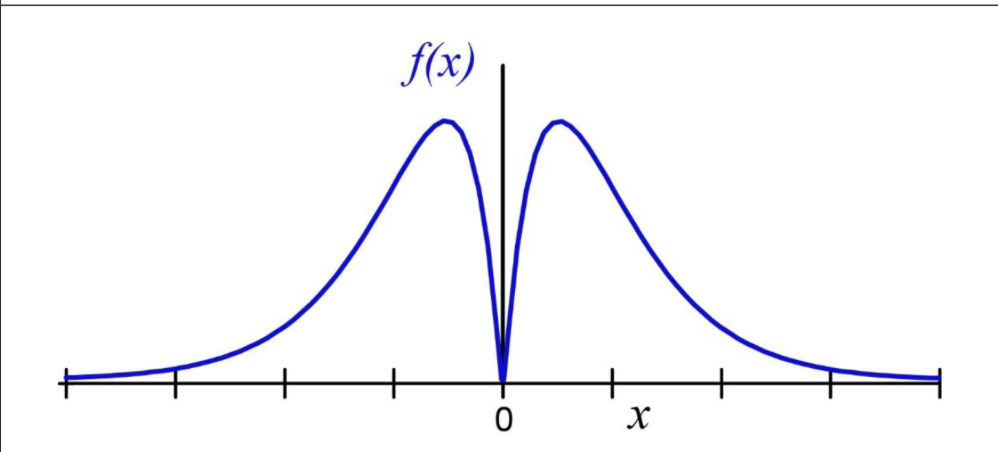
\includegraphics[width=0.5\columnwidth]{Figs/q7.png}
    \caption{Caption}
    \label{fig:placeholder}
\end{figure}
\begin{enumerate}


 \item $ f(x) = x^2 \, 2^{-|x|} $\\[0.8em]
\item  $ f(x) = x \, 2^{-|x|} $\\[0.8em]
\item $(x) = |x| \, 2^{-|x|} $\\[0.8em]
 \item $f(x) = x \, 2^{-x}$ \\
\end{enumerate}
     
     
>>>>>>> b031c34efd4dd324facb86a5e10db7b7cbd90dc1
  \item 
Which one of the following options can be inferred from the given passage alone?

\medskip

\noindent
\textbf{When I was a kid, I was partial to stories about other worlds and interplanetary travel. I used to imagine that I could just gaze off into space and be whisked to another planet.}\\
\hfill --- \textit{Excerpt from *The Truth about Stories* by T. King}

\medskip

\begin{enumerate}
    \item It is a child's description of what he or she likes.
    \item It is an adult's memory of what he or she liked as a child.
    \item The child in the passage read stories about interplanetary travel only in parts.
    \item It teaches us that stories
    \end{enumerate}
<<<<<<< HEAD
    \hfill{\brak{\text{GATE PE 2016}}}
=======
    \hfill{\brak{\text{GATE BM 2023}}}
>>>>>>> b031c34efd4dd324facb86a5e10db7b7cbd90dc1
    
  \item 
Out of 1000 individuals in a town, 100 unidentified individuals are covid positive. Due to lack of adequate covid-testing kits, the health authorities of the town devised a strategy to identify these covid-positive individuals. The strategy is to:

\begin{enumerate}[label=(\roman*)]
    \item Collect saliva samples from all 1000 individuals and randomly group them into sets of 5.
    \item Mix the samples within each set and test the mixed sample for covid.
    \item If the test done in (ii) gives a negative result, then declare all the 5 individuals to be covid negative.
    \item If the test done in (ii) gives a positive result, then all the 5 individuals are separately tested for covid.
\end{enumerate}

Given this strategy, no more than \rule{2cm}{0.15mm} testing kits will be required to identify all the 100 covid positive individuals irrespective of how they are grouped.



\begin{enumerate}
    \item 700
    \item 600
    \item 800
    \item 1000
    \end{enumerate}
<<<<<<< HEAD
    \hfill{\brak{\text{GATE PE 2016}}}
=======
    \hfill{\brak{\text{GATE BM 2023}}}
>>>>>>> b031c34efd4dd324facb86a5e10db7b7cbd90dc1
    
   \textbf {(10)}
A \(100 \, \text{cm} \times 32 \, \text{cm}\) rectangular sheet is folded 5 times. Each time the sheet is folded, the long edge aligns with its opposite side. Eventually, the folded sheet is a rectangle of dimensions \(100 \, \text{cm} \times 1 \, \text{cm}\).



The total number of creases visible when the sheet is unfolded is \rule{2cm}{0.15mm}.



\begin{enumerate}
    \item 32
    \item 5
    \item 31
    \item 63
\end{enumerate}
<<<<<<< HEAD
\hfill{\brak{\text{GATE PE 2016}}}
=======
\hfill{\brak{\text{GATE BM 2023}}}
>>>>>>> b031c34efd4dd324facb86a5e10db7b7cbd90dc1

\section*{Q.11 -- Q.35 Carry ONE mark Each}

\item  What is the magnitude of the difference between the mean and the median of the dataset \(\{1, 2, 3, 4, 6, 8\}\)?

\begin{enumerate}
    \item 0
    \item 1
    \item 0.5
    \item 0.25
\end{enumerate}
<<<<<<< HEAD
\hfill{\brak{\text{GATE PE 2016}}}
=======
\hfill{\brak{\text{GATE BM 2023}}}
>>>>>>> b031c34efd4dd324facb86a5e10db7b7cbd90dc1

 \item 
For a Binomial random variable \(X\), \(E(X)\) and \(\text{Var}(X)\) are the expectation and variance, respectively. Which one of the following statements \textbf{CANNOT} be true?

\begin{enumerate}
    \item \(E(X) = 20\) and \(\text{Var}(X) = 16\)
    \item \(E(X) = 6\) and \(\text{Var}(X) = 5.4\)
    \item \(E(X) = 10\) and \(\text{Var}(X) = 15\)
    \item \(E(X) = 64\) and \(\text{Var}(X) = 12.8\)
\end{enumerate}
<<<<<<< HEAD
\hfill{\brak{\text{GATE PE 2016}}}
=======
\hfill{\brak{\text{GATE BM 2023}}}
>>>>>>> b031c34efd4dd324facb86a5e10db7b7cbd90dc1

\textbf{(13)}

Let 
$
Q = \myvec{
1 & -2 \\
2 & 1
}
$
be a \(2 \times 2\) matrix. Which one of the following statements is \textbf{TRUE}?

\begin{enumerate}
    \item \(Q\) is equal to its transpose.
    \item \(Q\) is equal to its inverse.
    \item \(Q\) is of full rank.
    \item \(Q\) has linearly dependent columns.
\end{enumerate}
<<<<<<< HEAD
\hfill{\brak{\text{GATE PE 2016}}}
=======
\hfill{\brak{\text{GATE BM 2023}}}
>>>>>>> b031c34efd4dd324facb86a5e10db7b7cbd90dc1

\item 
Which one of the following vectors is an eigenvector corresponding to the eigenvalue \(\lambda = 1\) for the matrix \(A\)?
$
A = \myvec{
1 & -1 & 0 \\
1 & -1 & 1 \\
-1 & 0 & 1
}
$

\begin{enumerate}
    \item \([1 \;\; 0 \;\; 1]^T\)
    \item \([1 \;\; 1 \;\; 0]^T\)
    \item \([1 \;\; 0 \;\; 0]^T\)
    \item \([0 \;\; 0 \;\; 1]^T\)
\end{enumerate}
<<<<<<< HEAD
\hfill{\brak{\text{GATE PE 2016}}}
=======
\hfill{\brak{\text{GATE BM 2023}}}
>>>>>>> b031c34efd4dd324facb86a5e10db7b7cbd90dc1

\item 
For the function \( f(x, y) = e^x \cos(y) \), what is the value of 
$
\frac{\partial^2 f}{\partial x \partial y}
\text{ at } (x = 0, y = \frac{\pi}{2})?
$

\begin{enumerate}
    \item 0
    \item 1
    \item -1
    \item \( \frac{e}{2} \)
\end{enumerate}
<<<<<<< HEAD
\hfill{\brak{\text{GATE PE 2016}}}
=======
\hfill{\brak{\text{GATE BM 2023}}}
>>>>>>> b031c34efd4dd324facb86a5e10db7b7cbd90dc1

\item 
For the circuit given below, choose the angular frequency \(\omega_0\) (in rad/s) at which the voltage across the capacitor has maximum amplitude:

\begin{center}
\begin{circuitikz}[american]
    \draw (0,0)
    to[sV, l=\(100 \cos(\omega_0 t)\) Volts] (0,3)
    to[R, l=1\,k\(\Omega\)] (3,3)
    to[C, l=100\,\(\mu\)F] (3,0)
    -- (0,0);
\end{circuitikz}
\end{center}

\begin{enumerate}
    \item 1000
    \item 100
    \item 1
    \item 0
\end{enumerate}
<<<<<<< HEAD
\hfill{\brak{\text{GATE PE 2016}}}
=======
\hfill{\brak{\text{GATE BM 2023}}}
>>>>>>> b031c34efd4dd324facb86a5e10db7b7cbd90dc1

\item 
A finite impulse response (FIR) filter has only two non-zero samples in its impulse response \( h[n] \), namely \( h[0] = h[1] = 1 \). The Discrete Time Fourier Transform (DTFT) of \( h[n] \) equals \( H(e^{j\omega}) \), as a function of the normalized angular frequency \( \omega \). For the range \( |\omega| \leq \pi \), \( |H(e^{j\omega})| \) is equal to:

\begin{enumerate}
    \item \( 2|\cos(\omega)| \)
    \item \( 2|\sin(\omega)| \)
    \item \( 2|\cos(\omega/2)| \)
    \item \( 2|\sin(\omega/2)| \)
\end{enumerate}
<<<<<<< HEAD
\hfill{\brak{\text{GATE PE 2016}}}
=======
\hfill{\brak{\text{GATE BM 2023}}}
>>>>>>> b031c34efd4dd324facb86a5e10db7b7cbd90dc1

\item 
An 8-bit successive approximation Analog to Digital Converter (ADC) has a clock frequency of \( 1~\text{MHz} \). Assume that the start conversion and end conversion signals occupy one clock cycle each. Among the following options, what is the maximum frequency that this ADC can sample without aliasing?

\begin{enumerate}
    \item \( 0.9~\text{kHz} \)
    \item \( 9.9~\text{kHz} \)
    \item \( 49.9~\text{kHz} \)
    \item \( 99.9~\text{kHz} \)
\end{enumerate}
<<<<<<< HEAD
\hfill{\brak{\text{GATE PE 2016}}}
=======
\hfill{\brak{\text{GATE BM 2023}}}
>>>>>>> b031c34efd4dd324facb86a5e10db7b7cbd90dc1

\item 
In the following circuit with an ideal operational amplifier, the capacitance of the parallel plate capacitor \( C \) is given by the expression 
$
C = \left(\frac{\varepsilon A}{x}\right),
$
where \( \varepsilon \) is the dielectric constant of the medium between the capacitor plates, and \( A \) is the cross-sectional area. In the above relation, \( x \) is the separation between the two parallel plates, given by \( x = x_0 + kt \), where \( t \) is time; \( x_0 \) and \( k \) are positive non-zero constants. If the input voltage \( v_i \) is constant, then the output voltage \( v_o \) is given by

\begin{enumerate}
    \item \( Rv_i Ck \)
    \item \( \frac{Rv_i C}{kx} \)
    \item \( \frac{v_i k}{RCx} \)
    \item \(0\)
\end{enumerate}
<<<<<<< HEAD
\hfill{\brak{\text{GATE PE 2016}}}
=======
\hfill{\brak{\text{GATE BM 2023}}}
>>>>>>> b031c34efd4dd324facb86a5e10db7b7cbd90dc1

\item  Which one of the following techniques makes use of Korotkoff sounds?

\begin{enumerate}[label=(\Alph*)]
    \item Sphygmomanometry 
    \item Audiometry
    \item Spirometry
    \item Tonometry
\end{enumerate}
<<<<<<< HEAD
\hfill{\brak{\text{GATE PE 2016}}}
=======
\hfill{\brak{\text{GATE BM 2023}}}
>>>>>>> b031c34efd4dd324facb86a5e10db7b7cbd90dc1

\item  The pulmonary artery and pulmonary vein \underline{\hspace{3cm}}.
\begin{enumerate}[label=(\Alph*)]
    \item carry deoxygenated blood and oxygenated blood, respectively 
    \item carry oxygenated blood and deoxygenated blood, respectively
    \item both carry oxygenated blood
    \item both carry deoxygenated blood
\end{enumerate}
<<<<<<< HEAD
\hfill{\brak{\text{GATE PE 2016}}}
=======
\hfill{\brak{\text{GATE BM 2023}}}
>>>>>>> b031c34efd4dd324facb86a5e10db7b7cbd90dc1

\item  Which one of the following bridges \textbf{CANNOT} be used for measuring inductance?

\begin{enumerate}[label=(\Alph*)]
    \item Schering Bridge 
    \item Maxwell Wien Bridge
    \item Hay Bridge
    \item Series Owen Bridge
\end{enumerate}
<<<<<<< HEAD
\hfill{\brak{\text{GATE PE 2016}}}
=======
\hfill{\brak{\text{GATE BM 2023}}}
>>>>>>> b031c34efd4dd324facb86a5e10db7b7cbd90dc1


\item  A polychromatic beam of X-rays has an energy spectrum as shown in Figure P below. Which of the following graphs (in the options A to D) depicts the energy spectrum after passing through a human body? In each figure, the horizontal axis represents Energy in keV and the vertical axis represents Relative X-ray Intensity.
\begin{figure}[H]
\centering
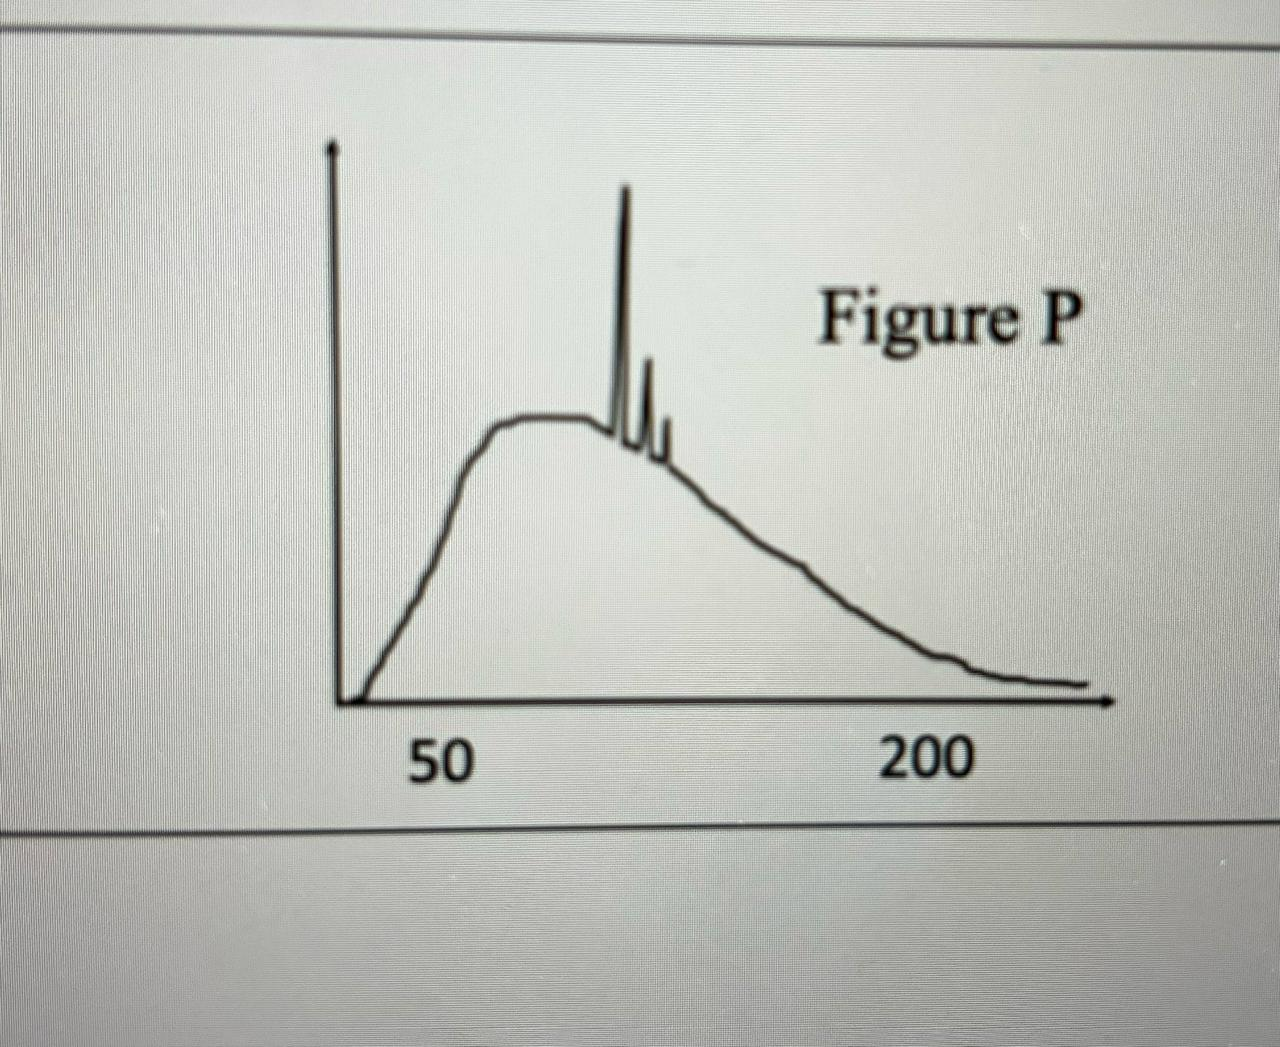
\includegraphics[width=0.4\columnwidth]{Figs/wavr.jpeg}
\caption{}
\end{figure}

\begin{figure}[H]
\centering
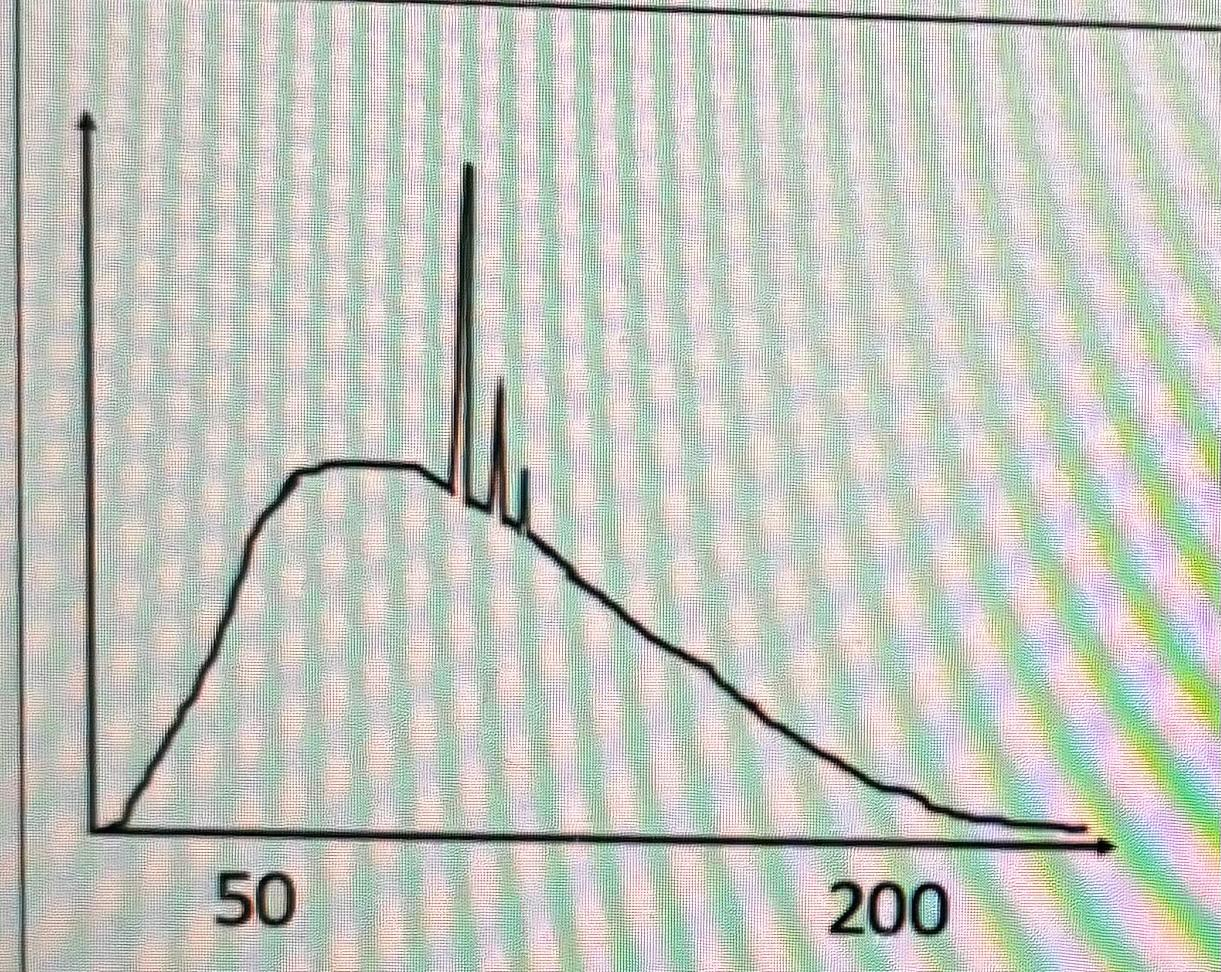
\includegraphics[width=0.4\columnwidth]{Figs/WAVE1.jpeg}
\caption{}
\end{figure}

\begin{figure}[H]
\centering
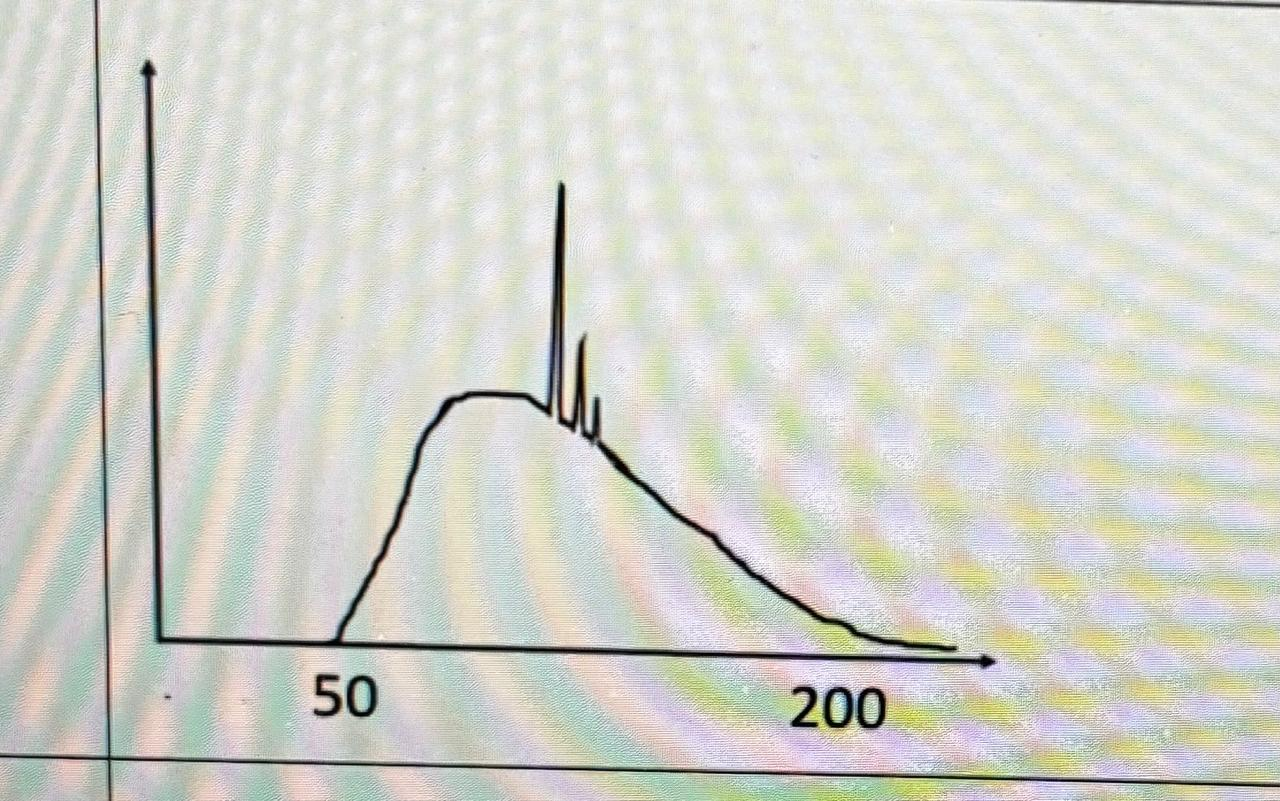
\includegraphics[width=0.4\columnwidth]{Figs/WAVE2.jpeg}
\caption{}
\end{figure}

\begin{figure}[H]
\centering
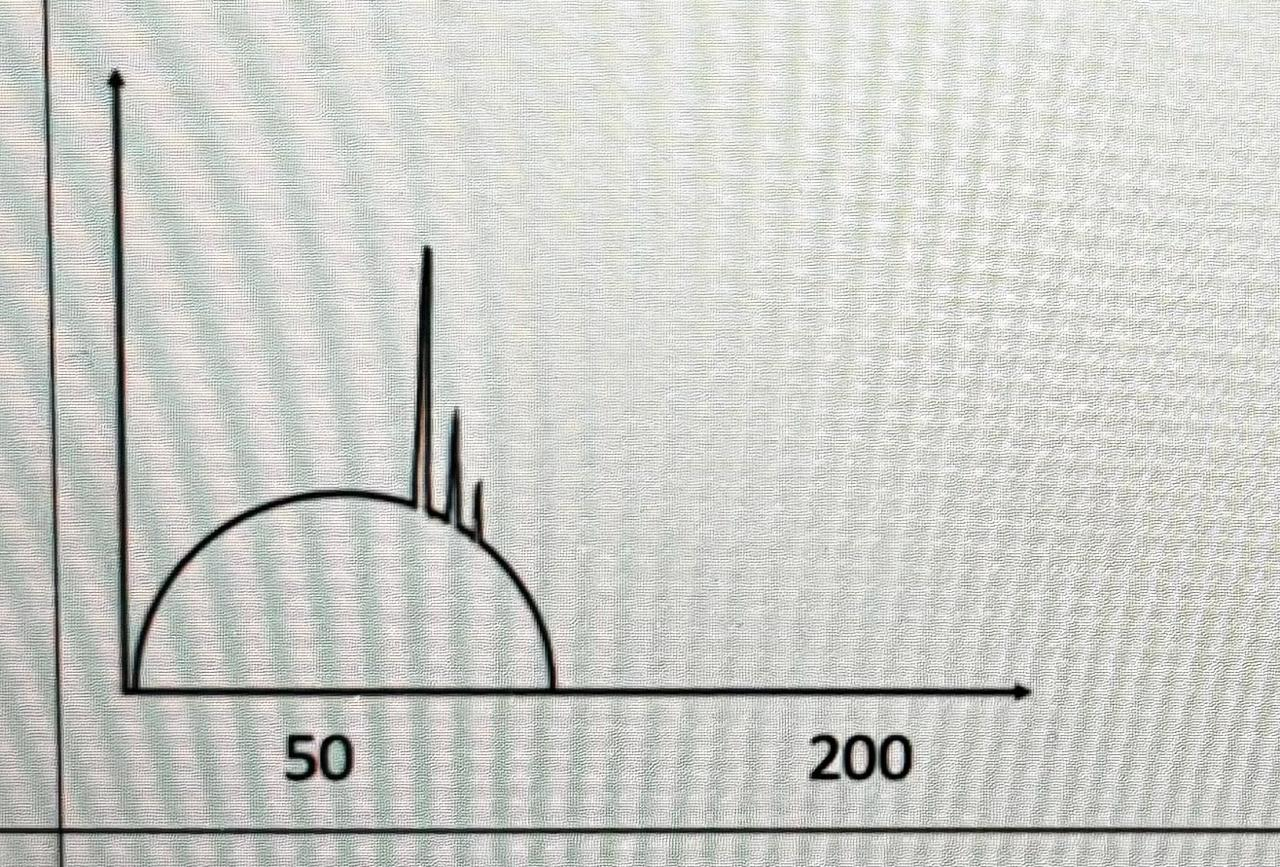
\includegraphics[width=0.4\columnwidth]{Figs/WAVE3.jpeg}
\caption{}
\end{figure}

\begin{figure}[H]
\centering
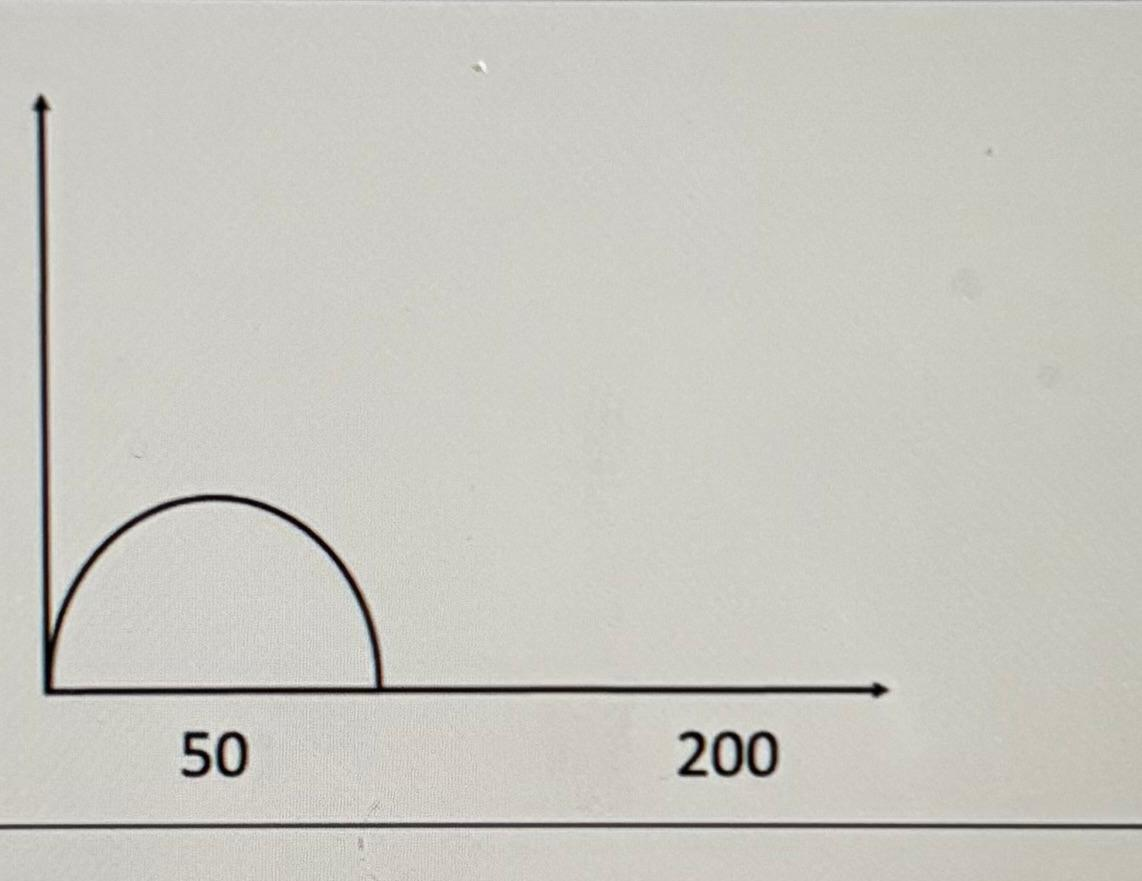
\includegraphics[width=0.4\columnwidth]{Figs/WAVE4.jpeg}
\caption{}
\end{figure}
<<<<<<< HEAD
\hfill{\brak{\text{GATE PE 2016}}}
=======
\hfill{\brak{\text{GATE BM 2023}}}
>>>>>>> b031c34efd4dd324facb86a5e10db7b7cbd90dc1

\item  \( M, L, T \) correspond to dimensions representing mass, length and time, respectively. What is the dimension of viscosity?

\begin{enumerate}
    \item \( M^1 L^{-2} T^{-1} \)
    \item \( M^1 L^{-1} T^{-1} \)
    \item \( M^1 L^{-1} T^{1} \)
    \item \( M^1 L^{-2} T^{-2} \)
\end{enumerate}
<<<<<<< HEAD
\hfill{\brak{\text{GATE PE 2016}}}
=======
\hfill{\brak{\text{GATE BM 2023}}}
>>>>>>> b031c34efd4dd324facb86a5e10db7b7cbd90dc1

\item  Choose the option that has the biomaterials arranged in order of decreasing tensile strength.

(PMMA: poly-methyl-methacrylate)

\begin{enumerate}
    \item Human compact bone $>$ PMMA bone cement $>$ Polymer foams $>$ Graphite-epoxy
    \item Human compact bone $>$ Graphite-epoxy $>$ PMMA bone cement $>$ Polymer foams
    \item Graphite-epoxy $>$ Human compact bone $>$ PMMA bone cement $>$ Polymer foams
    \item PMMA bone cement $>$ Human compact bone $>$ Polymer foams $>$ Graphite-epoxy
\end{enumerate}
<<<<<<< HEAD
\hfill{\brak{\text{GATE PE 2016}}}

\item  A causal, discrete time system is described by the difference equation
\[
y[n] = 0.5 \, y[n - 1] + x[n], \quad \text{for all } n,
\]
=======
\hfill{\brak{\text{GATE BM 2023}}}

\item  A causal, discrete time system is described by the difference equation
$
y[n] = 0.5 \, y[n - 1] + x[n], \quad \text{for all } n,
$
>>>>>>> b031c34efd4dd324facb86a5e10db7b7cbd90dc1
where \( y[n] \) denotes the output sequence and \( x[n] \) denotes the input sequence.
Which of the following statements is/are TRUE?

\begin{enumerate}
    \item The system has an impulse response described by \( 0.5^n \, u[n] \) where \( u[n] \) is the unit step sequence.
    \item The system is stable in the bounded input, bounded output sense.
    \item The system has an infinite number of non-zero samples in its impulse response.
    \item The system has a finite number of non-zero samples in its impulse response.
\end{enumerate}
<<<<<<< HEAD
\hfill{\brak{\text{GATE PE 2016}}}
=======
\hfill{\brak{\text{GATE BM 2023}}}
>>>>>>> b031c34efd4dd324facb86a5e10db7b7cbd90dc1

\item  Which of the following constituents is/are \textbf{NOT} normally found in serum obtained from human blood?

\begin{enumerate}
    \item Platelets
    \item Albumin
    \item Glucose
    \item Fibrinogen
\end{enumerate}
<<<<<<< HEAD
\hfill{\brak{\text{GATE PE 2016}}}
=======
\hfill{\brak{\text{GATE BM 2023}}}
>>>>>>> b031c34efd4dd324facb86a5e10db7b7cbd90dc1

\item  \( Q, R, S \) are Boolean variables and \( \oplus \) is the XOR operator. Select the CORRECT option(s):

\begin{enumerate}
    \item \( (Q \oplus R) \oplus S = Q \oplus (R \oplus S) \)
    \item \( (Q \oplus R) \oplus S = 0 \) when any two of the Boolean variables \( (Q, R, S) \) are 0 and the third variable is 1
    \item \( (Q \oplus R) \oplus S = 1 \) when \( Q = R = S = 1 \)
    \item \( ((Q \oplus R) \oplus (R \oplus S)) \oplus (Q \oplus S) = 1 \)
\end{enumerate}
<<<<<<< HEAD
\hfill{\brak{\text{GATE PE 2016}}}
=======
\hfill{\brak{\text{GATE BM 2023}}}
>>>>>>> b031c34efd4dd324facb86a5e10db7b7cbd90dc1

\item  In the human pancreas, which cell types secrete insulin and glucagon?

\begin{enumerate}
    \item Alpha cells and delta cells, respectively
    \item Beta cells and delta cells, respectively
    \item Alpha cells and beta cells, respectively
    \item Beta cells and alpha cells, respectively
\end{enumerate}
<<<<<<< HEAD
\hfill{\brak{\text{GATE PE 2016}}}
=======
\hfill{\brak{\text{GATE BM 2023}}}
>>>>>>> b031c34efd4dd324facb86a5e10db7b7cbd90dc1

\item  In the following circuit, the switch \( S \) is open for \( t < 0 \) and closed for \( t \geq 0 \). What is the steady state voltage (in Volts) across the capacitor when the switch is closed?\\
(Round off the answer to one decimal place.)
\begin{figure}[H]
    \centering
    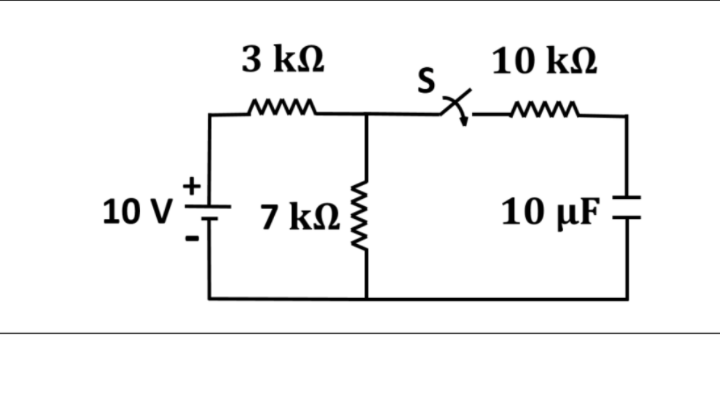
\includegraphics[width=0.5\columnwidth]{Figs/q28.png}
    \caption{Caption}
    \label{fig:placeholder}
\end{figure}
<<<<<<< HEAD
\hfill{\brak{\text{GATE PE 2016}}}

\item  For a tissue with Young's modulus of \SI{3.6}{\kilo\pascal} and Poisson's ratio of 0.2, what is the value of its shear modulus (in \si{\kilo\pascal})?
(Round off the answer to one decimal place.)
\hfill{\brak{\text{GATE PE 2016}}}
=======

\hfill{\brak{\text{GATE BM 2023}}}

\item  For a tissue with Young's modulus of \SI{3.6}{\kilo\pascal} and Poisson's ratio of 0.2, what is the value of its shear modulus (in \si{\kilo\pascal})?
(Round off the answer to one decimal place.)
\hfill{\brak{\text{GATE BM 2023}}}
>>>>>>> b031c34efd4dd324facb86a5e10db7b7cbd90dc1

\textbf{(32)} In the circuit shown below, the amplitudes of the voltage across the resistor and the capacitor are equal. What is the value of the angular frequency \( \omega_0 \) (in rad/s)?\\
(Round off the answer to one decimal place.)
\begin{center}
\begin{circuitikz}
    \draw
    (0,0) to[sinusoidal voltage source, l_=\(100 \cos(\omega_0 t) \text{ Volts}\)] (0,3)
    to[R, l=\(1\,\text{k}\Omega\)] (3,3)
    to[C, l=\(100\,\mu\text{F}\)] (3,0)
    -- (0,0);
\end{circuitikz}
\end{center}
<<<<<<< HEAD
\hfill{\brak{\text{GATE PE 2016}}}

\item  A continuous time, band limited signal \( x(t) \) has its Fourier transform described by:
\[
=======
\hfill{\brak{\text{GATE BM 2023}}}

\item  A continuous time, band limited signal \( x(t) \) has its Fourier transform described by:
$
>>>>>>> b031c34efd4dd324facb86a5e10db7b7cbd90dc1
X(f) =
\begin{cases}
1 - \dfrac{|f|}{200}, & \text{if } |f| \leq 200 \text{ Hz} \\
0, & \text{if } |f| > 200 \text{ Hz}
\end{cases}
$

The signal is uniformly sampled at a sampling rate of 600 Hz. The Fourier transform of the sampled signal is \( X_s(f) \). What is the value of \( \dfrac{X_s(600)}{X_s(500)} \)? (Round off the answer to one decimal place.)
<<<<<<< HEAD
\hfill{\brak{\text{GATE PE 2016}}}

\item  At time \( t \), the cardiac dipole is oriented at \(-45\degree\) (minus forty five degrees) to the horizontal axis. The magnitude of the dipole is \(3\ \text{mV}\). Assuming Einthoven frontal plane configuration, what is the magnitude (in mV) of the electrical signal in lead II? (Round off the answer to two decimal places.)
\hfill{\brak{\text{GATE PE 2016}}}

\textbf{(35)} A 5~MHz ultrasound transducer is being used to measure the velocity of blood. When the transducer is placed at an angle of \( 45\degree \) to the direction of blood flow, a frequency shift of 200~Hz is observed in the echo. Assume that the velocity of sound is 1500~m/s. What is the velocity (in cm/s) of the blood flow? (Round off the answer to one decimal place.)

\hfill{\brak{\text{GATE PE 2016}}}

\item  The time-dependent growth of a bacterial population is governed by the equation
\[
=======
\hfill{\brak{\text{GATE BM 2023}}}

\item  At time \( t \), the cardiac dipole is oriented at \(-45\degree\) (minus forty five degrees) to the horizontal axis. The magnitude of the dipole is \(3\ \text{mV}\). Assuming Einthoven frontal plane configuration, what is the magnitude (in mV) of the electrical signal in lead II? (Round off the answer to two decimal places.)
\hfill{\brak{\text{GATE BM 2023}}}

\textbf{(35)} A 5~MHz ultrasound transducer is being used to measure the velocity of blood. When the transducer is placed at an angle of \( 45\degree \) to the direction of blood flow, a frequency shift of 200~Hz is observed in the echo. Assume that the velocity of sound is 1500~m/s. What is the velocity (in cm/s) of the blood flow? (Round off the answer to one decimal place.)

\hfill{\brak{\text{GATE BM 2023}}}

\item  The time-dependent growth of a bacterial population is governed by the equation
$
>>>>>>> b031c34efd4dd324facb86a5e10db7b7cbd90dc1
\frac{dx}{dt} = x \left(1 - \frac{x}{200} \right),
$
where \( x \) is the population size at time \( t \). The initial population size is \( x_0 = 100 \) at \( t = 0 \). As \( t \to \infty \), the population size of bacteria asymptotically approaches \rule{4cm}{0.15mm}.

\begin{enumerate}
    \item 150
    \item 200
    \item 300
    \item 500
\end{enumerate}
<<<<<<< HEAD
\hfill{\brak{\text{GATE PE 2016}}}
=======
\hfill{\brak{\text{GATE BM 2023}}}
>>>>>>> b031c34efd4dd324facb86a5e10db7b7cbd90dc1

\item  
A \SI{20}{\milli\volt} DC signal has been superimposed with a \SI{10}{\milli\volt} RMS band-limited Gaussian noise with a flat spectrum up to \SI{5}{\kilo\hertz}. If an integrating voltmeter is used to measure this DC signal, what is the minimum averaging time (in seconds) required to yield a 99\% accurate result with 95\% certainty?

\begin{itemize}
  \item 0.1
  \item 1.0
  \item 5.0
  \item 10.0
\end{itemize}
<<<<<<< HEAD
\hfill{\brak{\text{GATE PE 2016}}}
=======
\hfill{\brak{\text{GATE BM 2023}}}
>>>>>>> b031c34efd4dd324facb86a5e10db7b7cbd90dc1

\item  
In the circuit below, the two DC voltage sources have voltages of value \( V_1 \) and \( V_2 \). 
The expression for the power dissipated in the \SI{60}{\kilo\ohm} resistor is proportional to \underline{\hspace{2cm}}.

\begin{center}
\begin{tabular}{c}
\begin{picture}(200,100)
% V1 source
\put(0,60){\makebox(0,0){$V_1$}}
\put(10,60){\line(1,0){40}} % horizontal wire from V1
\put(50,60){\line(0,-1){20}} % vertical down
\put(50,40){\makebox(0,0){\SI{10}{\kilo\ohm}}}
\put(50,30){\line(0,-1){20}} % vertical to 0

% Node and 60k resistor
\put(50,10){\line(1,0){40}} % to 60k
\put(90,10){\makebox(0,0){\SI{60}{\kilo\ohm}}}
\put(90,10){\line(1,0){40}}

% Top branch with 20k and V2
\put(130,10){\line(0,1){20}} % up
\put(130,30){\makebox(0,0){\SI{20}{\kilo\ohm}}}
\put(130,30){\line(0,1){30}} % up to V2
\put(130,60){\line(-1,0){120}} % back to V1 source

% V2 Source
\put(150,60){\makebox(0,0){$V_2$}}

\end{picture}
\end{tabular}
\end{center}

\textbf{Options:}
\begin{itemize}
    \item \( (V_1 + V_2)^2 \)
    \item \( (3V_1 + V_2)^2 \)
    \item \( (2V_1 + V_2)^2 \)
    \item \( (V_1 + 2V_2)^2 \)
\end{itemize}
<<<<<<< HEAD
\hfill{\brak{\text{GATE PE 2016}}}
=======
\hfill{\brak{\text{GATE BM 2023}}}
>>>>>>> b031c34efd4dd324facb86a5e10db7b7cbd90dc1

\item 

The Laplace transform of \( x_1(t) = e^{-t} u(t) \) is \( X_1(s) \), where \( u(t) \) is the unit step function. \\
The Laplace transform of \( x_2(t) = e^{t} u(-t) \) is \( X_2(s) \). Which one of the following statements is TRUE?

\begin{itemize}
    \item The region of convergence of \( X_1(s) \) is \( \mathrm{Re}(s) > 0 \).
    \item The region of convergence of \( X_2(s) \) is confined to the left half-plane of \( s \).
    \item The region of convergence of \( X_1(s) \) is confined to the right half-plane of \( s \).
    \item The imaginary axis in the \( s \)-plane is included in both the region of convergence of \( X_1(s) \) and the region of convergence of \( X_2(s) \).
\end{itemize}
<<<<<<< HEAD
\hfill{\brak{\text{GATE PE 2016}}}
=======
\hfill{\brak{\text{GATE BM 2023}}}
>>>>>>> b031c34efd4dd324facb86a5e10db7b7cbd90dc1

\item 
A circular disc of radius \( R \) (in cm) has a uniform absorption coefficient of \( 1 \, \text{cm}^{-1} \). 
Consider a single ray passing through the disc in the plane of the disc. The shortest distance from the center of the disc to the ray is \( t \) (in cm). 
If \( I_i \) is the intensity of the incident ray and \( I_0 \) is the intensity of the transmitted ray, then \( \log\left(\frac{I_i}{I_0}\right) \) is given by:

\begin{itemize}
    \item \( 2\sqrt{R^2 - t^2} \)
    \item \( 2R \)
    \item \( 1 \)
    \item \( 2\sqrt{R} - t \)
\end{itemize}
<<<<<<< HEAD
\hfill{\brak{\text{GATE PE 2016}}}
=======
\hfill{\brak{\text{GATE BM 2023}}}
>>>>>>> b031c34efd4dd324facb86a5e10db7b7cbd90dc1

\item  
The free induction decay (FID) in the MRI of an object can be approximated as:
$
s(t) = \iint m(x,y) e^{-j 2\pi \left(K_x(t)x + K_y(t)y\right)} \, dx \, dy,
$
where
$
K_x(t) = \int_0^t G_x(\tau)\, d\tau \quad \text{and} \quad K_y(t) = \int_0^t G_y(\tau)\, d\tau.
$

Here \( G_x \) and \( G_y \) are pulses of identical period and are in-phase. By changing the amplitude of the pulses, one can obtain the two dimensional Fourier transform of the object \underline{\hspace{2cm}}.

\begin{itemize}
    \item over radial lines in \( (K_x, K_y) \) space
    \item over a parabolic contour in \( (K_x, K_y) \) space
    \item along \( K_y \) only
    \item along \( K_x \) only
\end{itemize}
<<<<<<< HEAD
\hfill{\brak{\text{GATE PE 2016}}}

\item  
In the circuit shown below, it is observed that the amplitude of the voltage across the resistor is the same as the amplitude of the source voltage. What is the angular frequency \( \omega_0 \) (in rad/s)?
\hfill{\brak{\text{GATE PE 2016}}}
=======
\hfill{\brak{\text{GATE BM 2023}}}

\item  
In the circuit shown below, it is observed that the amplitude of the voltage across the resistor is the same as the amplitude of the source voltage. What is the angular frequency \( \omega_0 \) (in rad/s)?
\hfill{\brak{\text{GATE BM 2023}}}
>>>>>>> b031c34efd4dd324facb86a5e10db7b7cbd90dc1
\begin{center}
\begin{circuitikz}[american]
\draw
  (0,0) to[sinusoidal voltage source, l=\(100\cos(\omega_0 t)\text{ V}\)] (0,3)
  -- (2,3)
  to[R, l=10\,k$\Omega$] (4,3)
  to[L, l=10\,mH] (6,3)
  -- (6,0)
  to[C, l=1\,$\mu$F] (2,0)
  -- (0,0);
\end{circuitikz}
\end{center}

\begin{itemize}
    \item \(10^4\)
    \item \(10^3\)
    \item \(10^3\pi\)
    \item \(10^4\pi\)
\end{itemize}


\item  
In a biomaterial, formation of hydrogen bonds on alcoholic groups will lead to a \rule{3cm}{0.15mm}.
<<<<<<< HEAD
\hfill{\brak{\text{GATE PE 2016}}}
=======
\hfill{\brak{\text{GATE BM 2023}}}
>>>>>>> b031c34efd4dd324facb86a5e10db7b7cbd90dc1
\begin{itemize}
    \item shift in the infra-red peak around \(1700~\text{cm}^{-1}\)
    \item shift in the infra-red peak around \(2800~\text{cm}^{-1}\)
    \item broadening of the infra-red peak around \(3500~\text{cm}^{-1}\)
    \item disappearance of the infra-red peak around \(1700~\text{cm}^{-1}\)
\end{itemize}


\item  
In the circuit shown below, the input voltage is sinusoidal and \(2.5~\text{V}\) peak to peak. The capacitors are \(1~\mu\text{F}\) each. Assume that the knee voltage of the diodes is \(0~\text{V}\) and \(R_L\) is very large (almost infinite). Which one of the following options is closest to the peak to peak voltage across \(R_L\), after a large number of cycles?

\begin{figure}[H]
\centering
\resizebox{0.5\textwidth}{!}{%
\begin{circuitikz}
\tikzstyle{every node}=[font=\LARGE]
\draw (3,11.75) to[C] (3,11.75);
\draw (3.75,11.75) to[C,l={ \LARGE C1}] (5.75,11.75);
\draw (5.75,11.75) to[D,l={ \LARGE D2}] (7.75,11.75);
\draw (3.75,11.75) to[sinusoidal voltage source, sources/symbol/rotate=auto] (3.75,9.75);
\draw (3.75,9.75) to[short] (6.5,9.75);
\draw (6.5,9.75) to[short] (8.5,9.75);
\draw (7.5,9.75) to[C,l={ \LARGE C2}] (7.5,11.5);
\draw (7.75,11.75) to[short] (8.5,11.75);
\draw (7.5,11.75) to[short] (7.5,11);
\draw (8.5,11.75) to[R,l={ \LARGE RL}] (8.5,9.75);
\draw (5.5,10) to[D,l={ \LARGE D1}] (5.5,11.75);
\draw (5.5,10) to[short] (5.5,10.5);
\draw (5.5,9.75) to[short] (5.5,10.25);
\end{circuitikz}
}%

\label{fig:my_label}
\end{figure}
\begin{itemize}
    \item \(1.25~\text{V}\)
    \item \(2.50~\text{V}\)
    \item \(5.00~\text{V}\)
    \item \(10.0~\text{V}\)
\end{itemize}
<<<<<<< HEAD
\hfill{\brak{\text{GATE PE 2016}}}
=======
\hfill{\brak{\text{GATE BM 2023}}}
>>>>>>> b031c34efd4dd324facb86a5e10db7b7cbd90dc1

\item  
An ultrasound plane wave of amplitude \( P_0 \) hits the semi-infinite boundary of two media having acoustic impedances \( Z_1 \) and \( Z_2 \). The sum of the amplitudes of the reflected and the incident waves at the boundary is equal to 

\vspace{0.3cm}

\begin{itemize}
    \item \( \frac{2 P_0 Z_2}{Z_1 + Z_2} \)
    \item \( \frac{P_0 (Z_2 - Z_1)}{Z_1 + Z_2} \)
    \item \( \frac{P_0 Z_2}{Z_1} \)
    \item \( \frac{P_0 Z_1}{Z_1 + Z_2} \)
\end{itemize}
<<<<<<< HEAD
\hfill{\brak{\text{GATE PE 2016}}}
=======
\hfill{\brak{\text{GATE BM 2023}}}
>>>>>>> b031c34efd4dd324facb86a5e10db7b7cbd90dc1

\item 
In the circuit given below, what should be the value of the resistance $R$ for maximum dissipation of power in $R$?

\begin{figure}[H]
\centering
\resizebox{0.5\textwidth}{!}{%
\begin{circuitikz}
\tikzstyle{every node}=[font=\LARGE]
\draw (3,11.75) to[C] (3,11.75);
\draw (3.75,11.25) to[american voltage source,l={ \LARGE 10V}] (3.75,9.25);
\draw (3.75,11.25) to[R,l={ \LARGE 2K$\Omega$}] (5.75,11.25);
\draw (5.75,11.25) to[R,l={ \LARGE 3K$\Omega$}] (5.75,9.5);
\draw (5.75,11.25) to[R,l={ \LARGE 1K$\Omega$}] (8,11.25);
\draw (8,11.25) to[R,l={ \LARGE R}] (8,9.5);
\draw (3.75,9.25) to[short] (8,9.25);
\draw (8,9.25) to[short] (8,9.75);
\draw (5.75,9.25) to[short] (5.75,9.75);
\end{circuitikz}
}%

\label{fig:my_label}
\end{figure}

\bigskip

\begin{itemize}
    \item 1.2 k$\Omega$
    \item 2.2 k$\Omega$
    \item 3.2 k$\Omega$
    \item 4.2 k$\Omega$
\end{itemize}
<<<<<<< HEAD
\hfill{\brak{\text{GATE PE 2016}}}
=======
\hfill{\brak{\text{GATE BM 2023}}}
>>>>>>> b031c34efd4dd324facb86a5e10db7b7cbd90dc1

\item 
Two sequences \( x_1[n] \) and \( x_2[n] \) are described as follows:
$
x_1[0] = x_2[0] = 1
$
$
x_1[1] = x_2[2] = 2
$
$
x_1[2] = x_2[1] = 1
$

$
x_1[n] = x_2[n] = 0 \quad \text{for all } n < 0 \text{ and } n > 2
$

If \( x[n] \) is obtained by convolving \( x_1[n] \) with \( x_2[n] \), which of the following equations is/are \textbf{TRUE}?

\bigskip

\begin{itemize}
    \item \( x[2] = x[3] \)
    \item \( x[1] = 2 \)
    \item \( x[4] = 3 \)
    \item \( x[2] = 5 \)
\end{itemize}
<<<<<<< HEAD
\hfill{\brak{\text{GATE PE 2016}}}
=======
\hfill{\brak{\text{GATE BM 2023}}}
>>>>>>> b031c34efd4dd324facb86a5e10db7b7cbd90dc1

\item 
The function 
$
f(Z) = \frac{1}{Z - 1}
$
of a complex variable \( Z \) is integrated on a closed contour in an anti-clockwise direction. For which of the following contours does this integral have a non-zero value?



\begin{itemize}
    \item \( |Z - 1| = 0.01 \)
    \item \( |Z - 1| = 0.1 \)
    \item \( |Z - 3| = 5 \)
    \item \( |Z| = 2 \)
\end{itemize}
<<<<<<< HEAD
\hfill{\brak{\text{GATE PE 2016}}}
=======
\hfill{\brak{\text{GATE BM 2023}}}
>>>>>>> b031c34efd4dd324facb86a5e10db7b7cbd90dc1

\textbf{(49)}
The continuous time signal \( x(t) \) is described by
$
x(t) = 
\begin{cases}
1, & 0 \le t \le 1 \\
0, & \text{elsewhere}
\end{cases}
$

If \( y(t) \) represents \( x(t) \) convolved with itself, which of the following statements is/are TRUE?

\begin{itemize}
    \item \( y(t) = 0 \) for all \( t < 0 \)
    \item \( y(t) = 0 \) for all \( t > 1 \)
    \item \( y(t) = 0 \) for all \( t > 3 \)
    \item \( \displaystyle \int_{0.1}^{0.75} \frac{dy(t)}{dt} \, dt \ne 0 \)
\end{itemize}
<<<<<<< HEAD
\hfill{\brak{\text{GATE PE 2016}}}
=======
\hfill{\brak{\text{GATE BM 2023}}}
>>>>>>> b031c34efd4dd324facb86a5e10db7b7cbd90dc1

\item 
Which of the following relation(s) is/are \textbf{CORRECT} in terms of various lung volume measurements?

\begin{enumerate}[label=(\Alph*)]
    \item Vital capacity minus expiratory reserve volume equals inspiratory capacity.
    \item Vital capacity plus expiratory reserve volume equals inspiratory capacity.
    \item Total lung capacity equals the sum of inspiratory capacity and functional residual capacity.
    \item Functional residual capacity is the difference between expiratory reserve volume and residual volume.
\end{enumerate}
<<<<<<< HEAD
\hfill{\brak{\text{GATE PE 2016}}}
=======
\hfill{\brak{\text{GATE BM 2023}}}
>>>>>>> b031c34efd4dd324facb86a5e10db7b7cbd90dc1

\item 
Assuming the operational amplifier in the circuit shown below to be ideal, which of the following properties hold(s) TRUE for the circuit?

\begin{figure}[H]
\centering
\resizebox{0.5\textwidth}{!}{%
\begin{circuitikz}
\tikzstyle{every node}=[font=\LARGE]
\draw (3,11.75) to[C] (3,11.75);
\draw (5.75,11.75) node[op amp,scale=1, yscale=-1 ] (opamp2) {};
\draw (opamp2.+) to[short] (4.25,12.25);
\draw  (opamp2.-) to[short] (4.25,11.25);
\draw (6.95,11.75) to[short](7.25,11.75);
\draw (4.25,12.75) to[short] (4.25,12.25);
\draw (4.25,12.75) to[short] (4.25,13.25);
\draw (4.25,13.25) to[short] (6.25,13.25);
\draw (6.25,13.25) to[short] (7.25,13.25);
\draw (7.25,13.25) to[short] (7.25,11.75);
\draw (4.25,11.25) to (4.25,10.5) node[sground]{};
\end{circuitikz}
}%

\label{fig:my_label}
\end{figure}

\begin{enumerate}[label=(\Alph*)]
    \item It acts as a voltage follower.
    \item It is bistable.
    \item It is astable.
    \item The output voltage is at saturation.
\end{enumerate}
<<<<<<< HEAD
\hfill{\brak{\text{GATE PE 2016}}}
=======
\hfill{\brak{\text{GATE BM 2023}}}
>>>>>>> b031c34efd4dd324facb86a5e10db7b7cbd90dc1
 \item 
 
A water insoluble polymeric biomaterial can become water soluble \textit{in vivo} by which of the following mechanisms?

\begin{enumerate}[label=(\Alph*)]
    \item Cleavage of crosslinks between water soluble polymer chains
    \item Cleavage of side chains leading to formation of non-polar groups
    \item Cleavage of backbone linkages between polymer repeat units leading to the formation of polar groups
    \item Enzymatic degradation of crosslinks between water soluble polymer chains
\end{enumerate}
<<<<<<< HEAD
\hfill{\brak{\text{GATE PE 2016}}}
=======
\hfill{\brak{\text{GATE BM 2023}}}
>>>>>>> b031c34efd4dd324facb86a5e10db7b7cbd90dc1

\item 
For the function \( f(x) = x^4 - x^2 \), which of the following statements is/are TRUE?

\begin{enumerate}[label=(\Alph*)]
    \item The function is symmetric about \( x = 0 \).
    \item The minimum value of the function is \( -0.5 \).
    \item The function has two minima.
    \item The function is an odd function.
\end{enumerate}
<<<<<<< HEAD
\hfill{\brak{\text{GATE PE 2016}}}
=======
\hfill{\brak{\text{GATE BM 2023}}}
>>>>>>> b031c34efd4dd324facb86a5e10db7b7cbd90dc1

\item 
A system is described by the following differential equation:
$
0.01 \frac{d^2 y(t)}{dt^2} + 0.2 \frac{dy(t)}{dt} + y(t) = 6x(t),
$
where time \( t \) is in seconds.

If \( x(t) \) is the unit step input applied at \( t = 0 \) s to this system, the magnitude of the output at \( t = 1 \) s is \underline{\hspace{3cm}}. 
(Round off the answer to two decimal places.)
<<<<<<< HEAD
\hfill{\brak{\text{GATE PE 2016}}}

\item  
The resistance of a thermistor is $1 \, \text{k}\Omega$ at $25^{\circ}\text{C}$ and $500 \, \Omega$ at $50^{\circ}\text{C}$. Find the temperature coefficient of resistance (in units of $^{\circ}\text{C}^{-1}$) at $35^{\circ}\text{C}$. (Round off the answer to three decimal places.)
\hfill{\brak{\text{GATE PE 2016}}}
=======
\hfill{\brak{\text{GATE BM 2023}}}

\item  
The resistance of a thermistor is $1 \, \text{k}\Omega$ at $25^{\circ}\text{C}$ and $500 \, \Omega$ at $50^{\circ}\text{C}$. Find the temperature coefficient of resistance (in units of $^{\circ}\text{C}^{-1}$) at $35^{\circ}\text{C}$. (Round off the answer to three decimal places.)
\hfill{\brak{\text{GATE BM 2023}}}
>>>>>>> b031c34efd4dd324facb86a5e10db7b7cbd90dc1

\item 
A normally incident X-ray of energy 140 keV passes through a tissue phantom and is detected by the detector as shown in the figure below. The phantom consists of tissue P with an absorption coefficient of \( 1\, \text{cm}^{-1} \) and a thickness of \( 1\, \text{cm} \), and tissue Q with an absorption coefficient of \( 10\, \text{cm}^{-1} \) and a thickness of \( 2\, \text{cm} \).

Calculate the intensity (in \(\mu\text{eV}\)) detected by the detector. 
\textit{(Round off the answer to one decimal place.)}

\begin{figure}
    \centering
    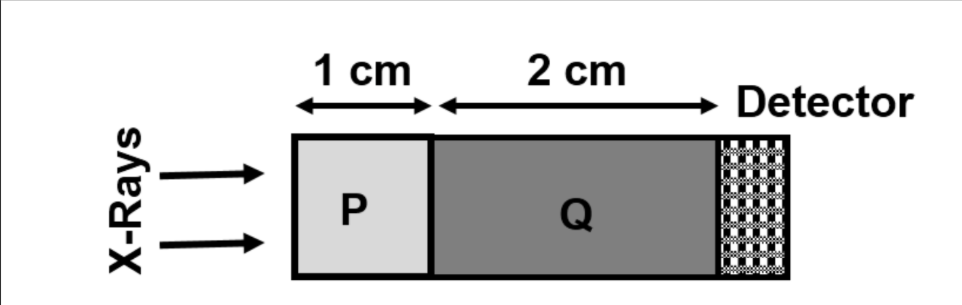
\includegraphics[width=0.5\columnwidth]{Figs/q56.png}
    \caption{Caption}
    \label{fig:placeholder}
\end{figure}

<<<<<<< HEAD
\begin{center}
\begin{tikzpicture}[scale=1]
  % Tissues
  \draw[thick] (0,0) rectangle (2,1); % Tissue P
  \node at (1,0.5) {P};
  \draw[thick, fill=gray!40] (2,0) rectangle (6,1); % Tissue Q
  \node at (4,0.5) {Q};
  
  % Detector
  \draw[thick, pattern=north east lines] (6,0) rectangle (6.8,1);
  \node[rotate=90] at (6.65,0.5) {Detector};
  
  % X-ray arrows
  \draw[->, thick] (-1,0.25) -- (0,0.25);
  \draw[->, thick] (-1,0.5) -- (0,0.5);
  \draw[->, thick] (-1,0.75) -- (0,0.75);
  \node at (-1.3,0.5) {X-Rays};
  
  % Dimension lines
  \draw[<->] (0,-0.2) -- (2,-0.2);
  \node at (1,-0.4) {1 cm};
  \draw[<->] (2,-0.2) -- (6,-0.2);
  \node at (4,-0.4) {2 cm};
\end{tikzpicture}
\end{center}
\hfill{\brak{\text{GATE PE 2016}}}

=======

  
\hfill{\brak{\text{GATE BM 2023}}}

>>>>>>> b031c34efd4dd324facb86a5e10db7b7cbd90dc1
\item 
A two-dimensional square plate (20 mm sides) contains a homogeneous circular inclusion of 5 mm diameter in it. A parallel beam of X-rays (beam width 30 mm) is used in a tomography system to determine the location of the inclusion. 

What is the \textbf{minimum number of views} required to approximately determine the location of the inclusion?
<<<<<<< HEAD
\hfill{\brak{\text{GATE PE 2016}}}
=======
\hfill{\brak{\text{GATE BM 2023}}}
>>>>>>> b031c34efd4dd324facb86a5e10db7b7cbd90dc1

\item 
Calculate the reciprocal of the coefficient of \( z^3 \) in the Taylor series expansion of the function 




around \( z = 0 \). (Provide the answer as an integer.)

<<<<<<< HEAD
\hfill{\brak{\text{GATE PE 2016}}}
=======
\hfill{\brak{\text{GATE BM 2023}}}
>>>>>>> b031c34efd4dd324facb86a5e10db7b7cbd90dc1

\item 
In a cell viability experiment, 10,000 cells were cultured in the absence and presence of a compound Q for 24 h. The absorbance of a dye associated with cellular metabolic activity was measured at a wavelength of 570 nm at 24 h. The measured absorbances were 0.8 a.u. in the absence of the compound Q, and 0.5 a.u. in its presence.

\vspace{0.5em}
If the dye gives an absorbance (at 570 nm) of 0.1 a.u. in the absence of cells, what is the percentage cell growth inhibition caused by the compound Q? (Round off the answer to one decimal place.)
<<<<<<< HEAD
\hfill{\brak{\text{GATE PE 2016}}}
=======
\hfill{\brak{\text{GATE BM 2023}}}
>>>>>>> b031c34efd4dd324facb86a5e10db7b7cbd90dc1


The volume percentage of oxygen in inspired air is 20\% and that of expired air is 16\%. A person is breathing at a rate of 12 breaths per minute. Each breath is 500 ml in volume. The cardiac output is 5 liters per minute.

\vspace{0.5em}
Assuming ideal, healthy lung and cardiac conditions, what is the change in percentage of oxygen in blood over 1 minute? (Round off the answer to one decimal place.)

<<<<<<< HEAD
\hfill{\brak{\text{GATE PE 2016}}}
=======
\hfill{\brak{\text{GATE BM 2023}}}
>>>>>>> b031c34efd4dd324facb86a5e10db7b7cbd90dc1

\item 
The intracellular and extracellular concentrations (in mM) of three important ions are given in the table below. The relative permeability of the cell membrane to each ion is provided. Universal gas constant is \( 8.31 \, \text{J/(mol.K)} \) and Faraday's constant is \( 96500 \, \text{C/mol} \).
What is the absolute value of the resting membrane potential (in mV) across the cell membrane at \( 27^\circ \text{C} \)? (Round off the answer to one decimal place.)

\begin{figure}[H]
    \centering
    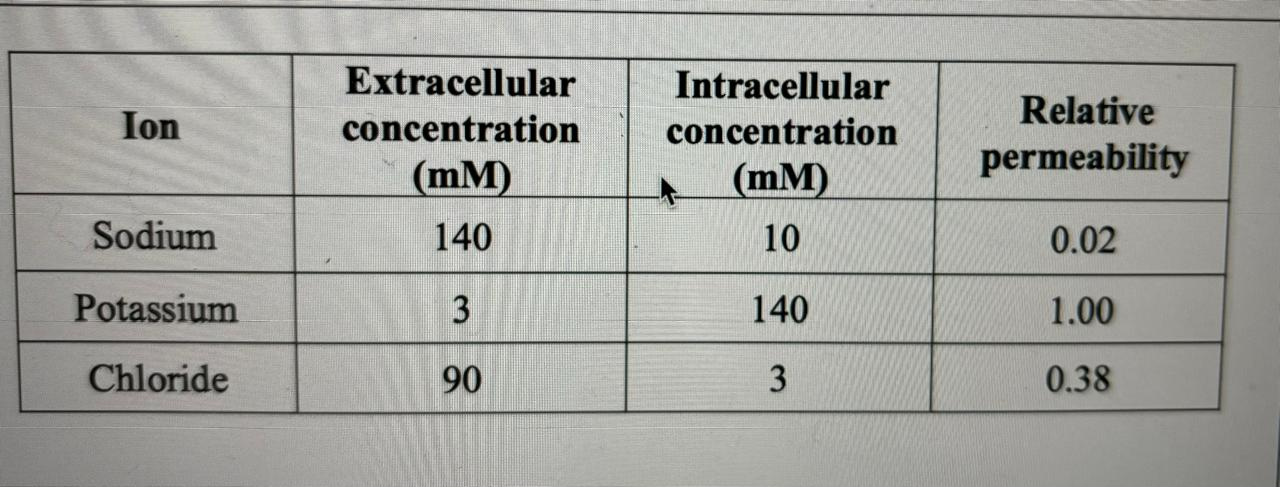
\includegraphics[width=1\columnwidth]{Figs/ASSIGN.jpeg}
    \caption{}
    \label{fig:placeholder}
\end{figure}
<<<<<<< HEAD
\hfill{\brak{\text{GATE PE 2016}}}


A metallic strain gauge with negligible piezoresistive effect is subjected to a strain of \( 50 \times 10^{-6} \). For the metal, Young's Modulus = \( 80 \, \text{GPa} \) and Poisson's Ratio = \( 0.42 \). What is the change in resistance (in m\(\Omega\)), if the unstrained resistance of the strain gauge is \( 200 \, \Omega \)? (Round off the answer to one decimal place.)
\hfill{\brak{\text{GATE PE 2016}}}
=======
\hfill{\brak{\text{GATE BM 2023}}}


A metallic strain gauge with negligible piezoresistive effect is subjected to a strain of \( 50 \times 10^{-6} \). For the metal, Young's Modulus = \( 80 \, \text{GPa} \) and Poisson's Ratio = \( 0.42 \). What is the change in resistance (in m\(\Omega\)), if the unstrained resistance of the strain gauge is \( 200 \, \Omega \)? (Round off the answer to one decimal place.)
\hfill{\brak{\text{GATE BM 2023}}}
>>>>>>> b031c34efd4dd324facb86a5e10db7b7cbd90dc1

\item 
Consider the total hip joint prosthesis as shown in the figure. The geometric parameters of the prosthesis are such that 
\( L_1 = 40 \, \text{mm}, \, L_2 = 60 \, \text{mm}, \, \theta_1 = 45^\circ, \, \theta_2 = 90^\circ \). 

Assume that, when standing symmetrically on both feet, a joint reaction force of \( 400 \, \text{N} \) is acting vertically at the femoral head (point A) due to the body weight of the subject. 

Calculate the magnitude of the moment (in Nm) about point C. (Round off the answer to one decimal place.)


\textbf{Diagram description:}

\begin{itemize}
  \item Point A is the femoral head (top).
  \item Segment \( AB \) has length \( L_1 \) and makes an angle \( \theta_1 = 45^\circ \) with the horizontal.
  \item Segment \( BC \) has length \( L_2 \) and is vertical (\( \theta_2 = 90^\circ \)).
  \item A vertical joint reaction force of \( 400 \, \text{N} \) acts downward at point A.
\end{itemize}
<<<<<<< HEAD
\hfill{\brak{\text{GATE PE 2016}}}
=======
\hfill{\brak{\text{GATE BM 2023}}}
>>>>>>> b031c34efd4dd324facb86a5e10db7b7cbd90dc1

\item 
A Wheatstone bridge strain gauge transducer is constructed on a diaphragm in such a way that when a force is applied on the diaphragm, the resistors \( R_1 \) and \( R_4 \) will be in compression, and the resistors \( R_2 \) and \( R_3 \) will be in tension.

\vspace{1em}
The bridge excitation voltage (\( E_{\text{in}} \)) is 10 Volts. If all the resistors have a resistance of \( 200 \, \Omega \) in the absence of any force, and each resistance changes by \( 20 \, \Omega \) upon application of a force, what is the output voltage \( V_{\text{out}} \) (in Volts) from the Wheatstone bridge? 

(Round off your answer to the nearest integer.)
\begin{figure}[H]
    \centering
    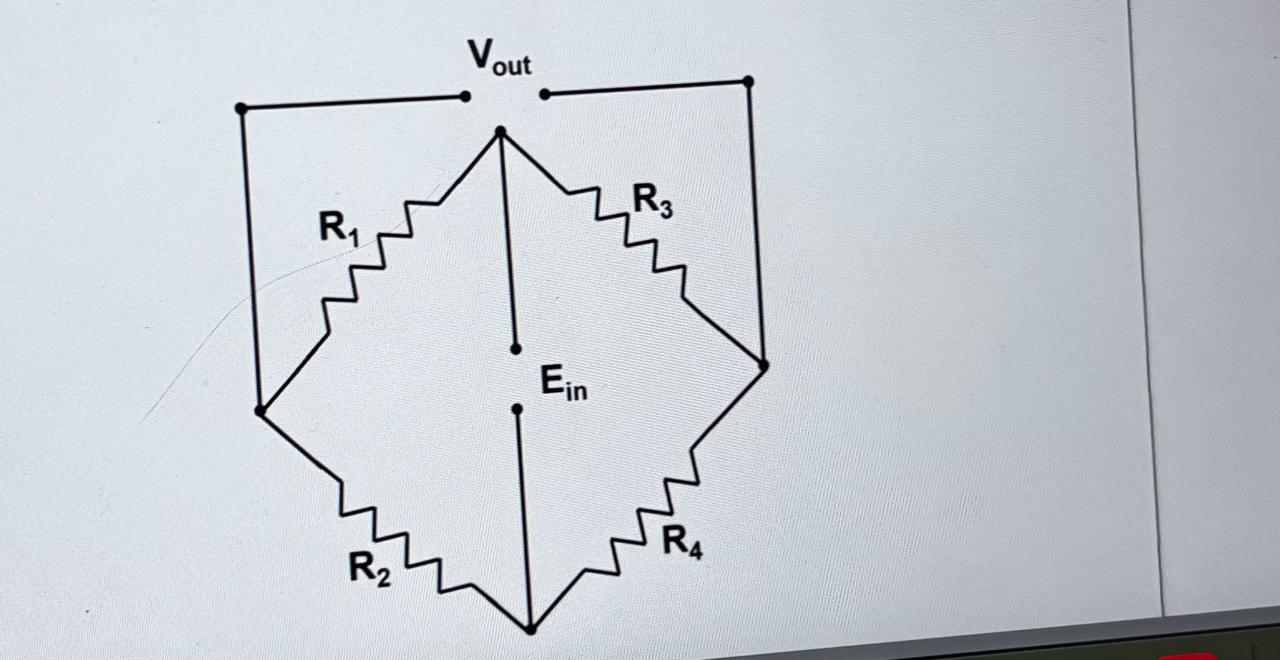
\includegraphics[width=0.5\columnwidth]{Figs/wheatstone.jpeg} 
    \caption{}
    \label{fig:placeholder}
\end{figure}
<<<<<<< HEAD
\hfill{\brak{\text{GATE PE 2016}}}
=======
\hfill{\brak{\text{GATE BM 2023}}}
>>>>>>> b031c34efd4dd324facb86a5e10db7b7cbd90dc1

\item 
A stone is thrown from an elevation of 2 m above ground level, at an angle of \(30^\circ\) to the horizontal axis. If the stone hits the ground at a horizontal distance of 6 m from the point of release, at what speed (in m/s) was the stone thrown? Use \(g = 10~\text{m/s}^2\) and assume that there is no air resistance. (Round off your answer to one decimal place.)

\begin{tikzpicture}[scale=1.2]

% Ground line
\draw[thick] (0,0) -- (7,0);

% Launch point
\filldraw[black] (0,2) circle (2pt);
\node[left] at (0,2) {2 m};

% Dashed trajectory arc
\draw[dashed,thick,->] (0,2) .. controls (2,3.5) and (4,3.5) .. (6,0);

% Horizontal distance arrow
\draw[<->] (0,-0.5) -- (6,-0.5);
\node at (3,-0.9) {6 m};

% Launch angle indicator
\draw[->,thick] (0,2) -- (1.8,2.9);
\draw (0.8,2) arc[start angle=0,end angle=30,radius=0.8];
\node at (1.1,2.25) {\small $30^\circ$};

% Axes and helpers
\draw[dotted] (0,2) -- (0,0);
\end{tikzpicture}

<<<<<<< HEAD
\hfill{\brak{\text{GATE PE 2016}}}
=======
\hfill{\brak{\text{GATE BM 2023}}}
>>>>>>> b031c34efd4dd324facb86a5e10db7b7cbd90dc1
\end{enumerate}
\end{document}